\documentclass[12pt,a4paper]{article}
%\usepackage{ctex}
\usepackage{amsmath,amscd,amsbsy,amssymb,latexsym,url,bm,amsthm}
\usepackage{epsfig,graphicx,subfigure}
\usepackage{enumitem,balance}
\usepackage{wrapfig}
\usepackage{mathrsfs,euscript}
\usepackage[x11names,svgnames,dvipsnames]{xcolor}
\usepackage{hyperref}
\usepackage[vlined,ruled,commentsnumbered,linesnumbered]{algorithm2e}
\usepackage{listings}
\usepackage{multicol}
%\usepackage{fontspec}

\renewcommand{\listalgorithmcfname}{List of Algorithms}
\renewcommand{\algorithmcfname}{Alg}

\newtheorem{theorem}{Theorem}
\newtheorem{lemma}[theorem]{Lemma}
\newtheorem{proposition}[theorem]{Proposition}
\newtheorem{corollary}[theorem]{Corollary}
\newtheorem{exercise}{Exercise}
\newtheorem*{solution}{Solution}
\newtheorem{definition}{Definition}
\theoremstyle{definition}


%\numberwithin{equation}{section}
%\numberwithin{figure}{section}

\renewcommand{\thefootnote}{\fnsymbol{footnote}}

\newcommand{\postscript}[2]
 {\setlength{\epsfxsize}{#2\hsize}
  \centerline{\epsfbox{#1}}}

\renewcommand{\baselinestretch}{1.0}

\setlength{\oddsidemargin}{-0.365in}
\setlength{\evensidemargin}{-0.365in}
\setlength{\topmargin}{-0.3in}
\setlength{\headheight}{0in}
\setlength{\headsep}{0in}
\setlength{\textheight}{10.1in}
\setlength{\textwidth}{7in}
\makeatletter \renewenvironment{proof}[1][Proof] {\par\pushQED{\qed}\normalfont\topsep6\p@\@plus6\p@\relax\trivlist\item[\hskip\labelsep\bfseries#1\@addpunct{.}]\ignorespaces}{\popQED\endtrivlist\@endpefalse} \makeatother
\makeatletter
\renewenvironment{solution}[1][Solution] {\par\pushQED{\qed}\normalfont\topsep6\p@\@plus6\p@\relax\trivlist\item[\hskip\labelsep\bfseries#1\@addpunct{.}]\ignorespaces}{\popQED\endtrivlist\@endpefalse} \makeatother


\definecolor{codegreen}{rgb}{0.44,0.68,0.28}
\definecolor{codegray}{rgb}{0.5,0.5,0.5}
\definecolor{codepurple}{rgb}{0.58,0,0.82}
\definecolor{backcolour}{rgb}{0.96,0.96,0.96}

\lstset{
language=C++,
frame=shadowbox,
keywordstyle = \color{blue}\bfseries,
commentstyle=\color{codegreen},
tabsize = 4,
backgroundcolor=\color{backcolour},
numbers=left,
numbersep=5pt,
breaklines=true,
emph = {int,float,double,char},emphstyle=\color{orange},
emph ={[2]const, typedef},emphstyle = {[2]\color{red}} }



\begin{document}
\noindent

%========================================================================
\noindent\framebox[\linewidth]{\shortstack[c]{
\Large{\textbf{Lab04-Hashing}}\vspace{1mm}\\
VE281 - Data Structures and Algorithms, Xiaofeng Gao, TA: Qingmin Liu, Autumn 2019}}
%CS26019 - Algorithm Design and Analysis, Xiaofeng Gao, Autumn 2019}}
\begin{center}
\footnotesize{\color{red}$*$ Please upload your assignment to website. Contact webmaster for any questions.}

\footnotesize{\color{blue}$*$ Name: Sun Yiwen  \quad Student ID: 517370910213 \quad Email: sunyw99@sjtu.edu.cn}
\end{center}


\begin{enumerate}

\item  Given a sequence of inputs 192, 42, 142, 56, 39, 319, 14, insert them
into a hash table of size 10. Suppose that the hash function is $h(x) = x\%10$. Show the
result for the following implementations:
	\begin{enumerate}
	\item Hash table using separate chaining. Assume that the insertion is always at the
beginning of each linked list.\\
	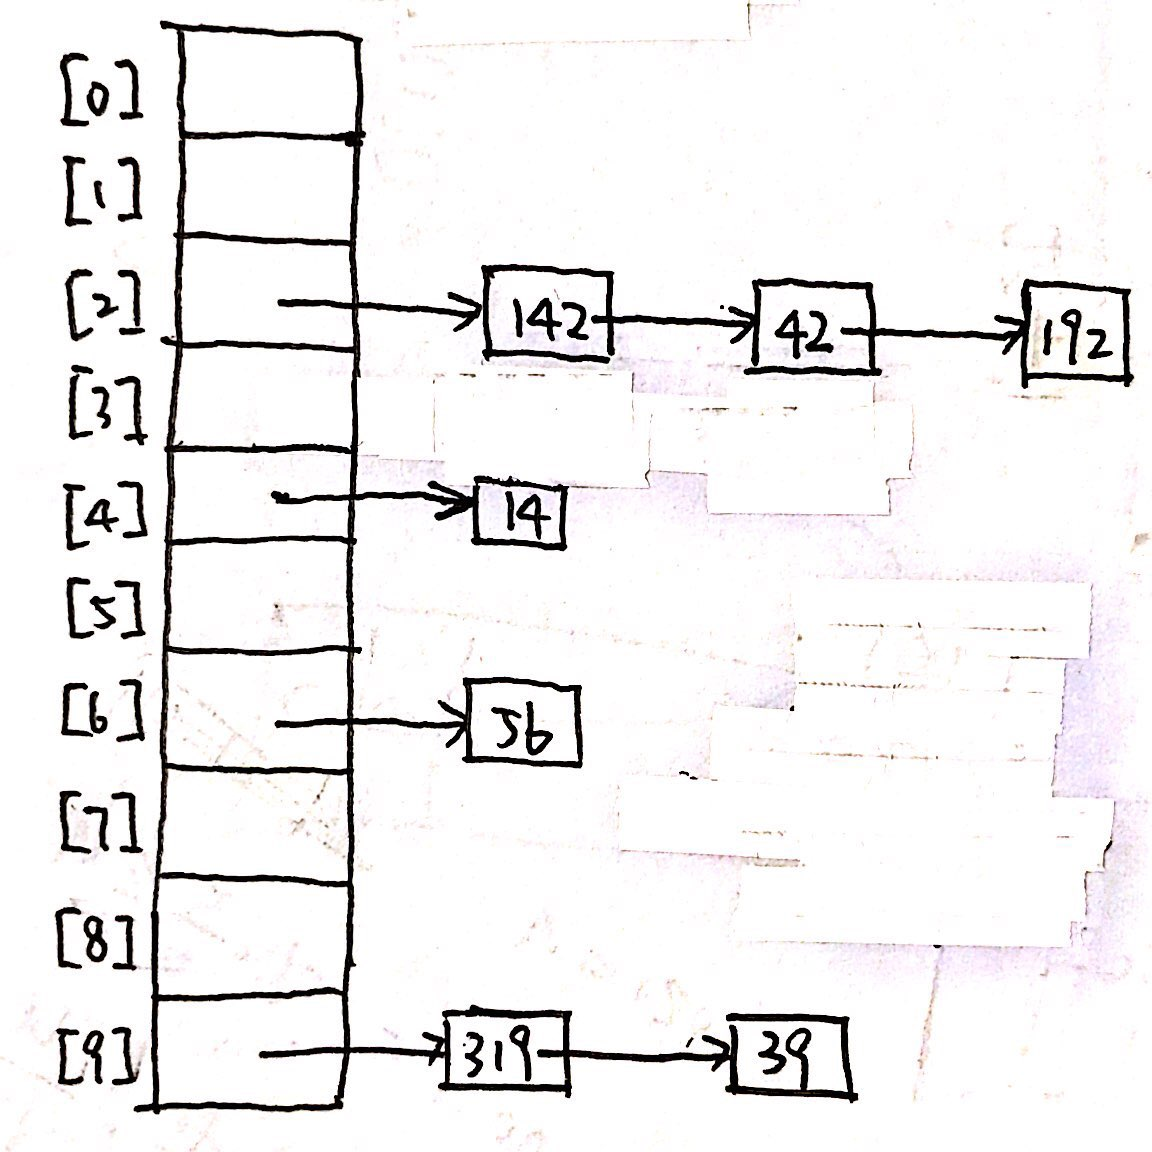
\includegraphics[scale=0.12]{f1.jpg}
	\item Hash table using linear probing.\\
	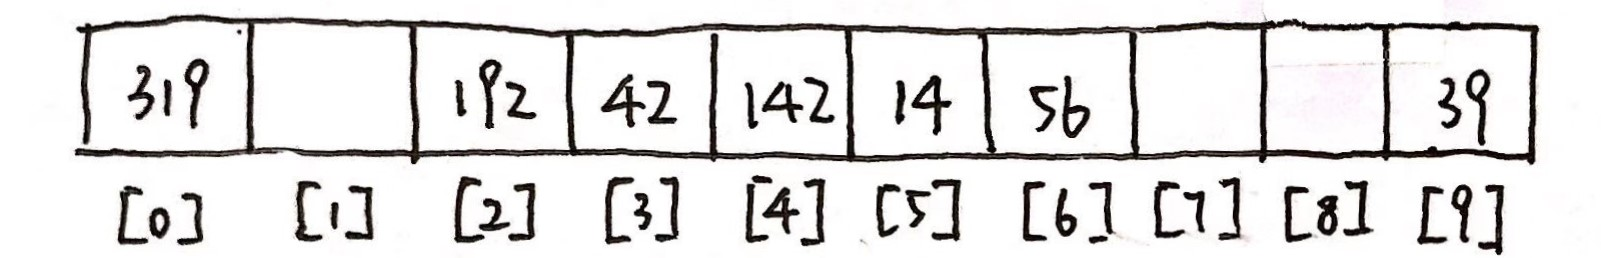
\includegraphics[scale=0.14]{f2.jpg}
	\item Hash table using quadratic probing.\\
	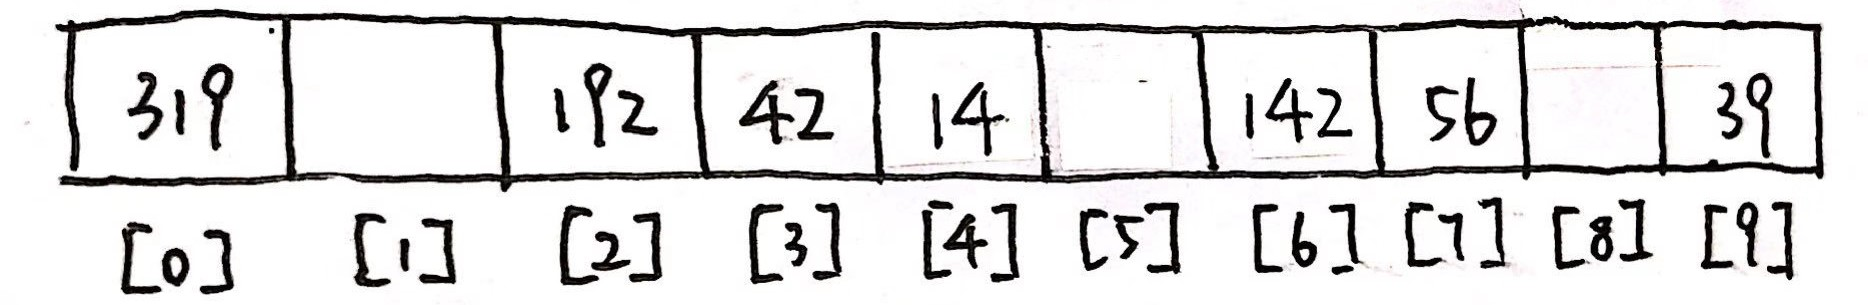
\includegraphics[scale=0.12]{f3.jpg}
	\item Hash table using double hashing, with the second hash function as $h_2 (x) = (x+4)\%7$.\\
	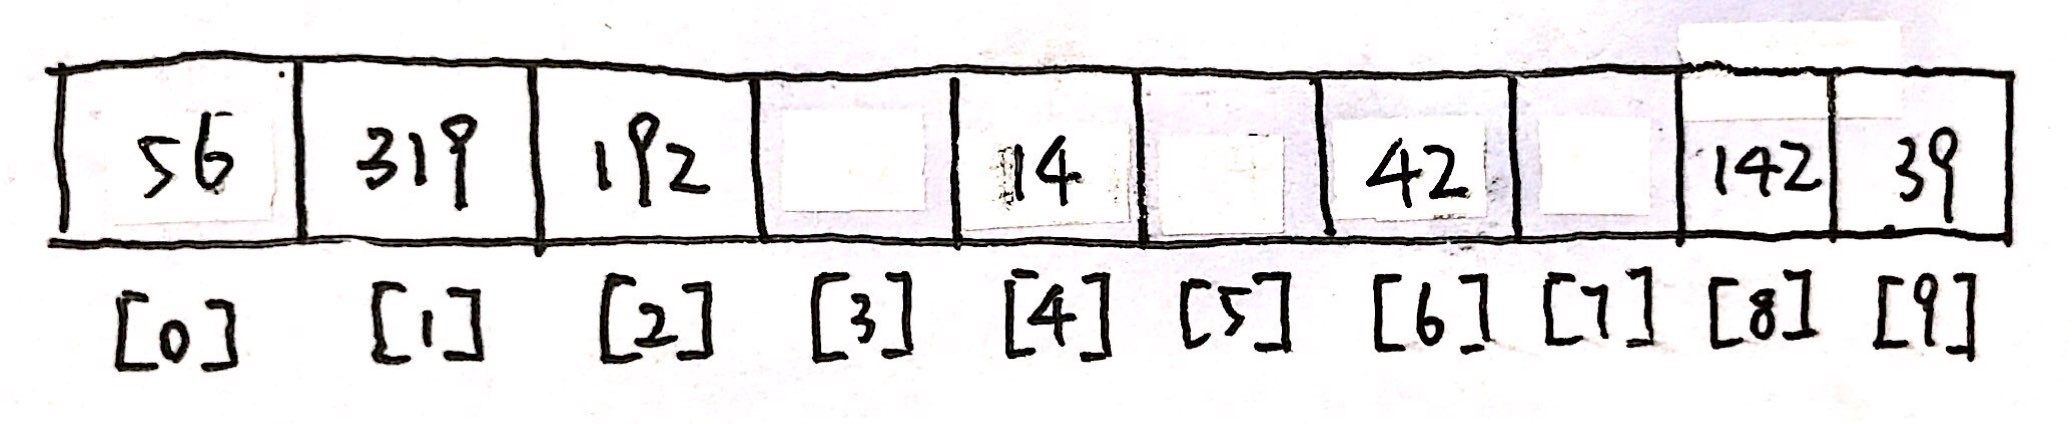
\includegraphics[scale=0.11]{f4.jpg}

	
	\end{enumerate}
\item	 Show the result of rehashing the four hash tables in the Problem 1. Rehash
using a new table size of 14, and a new hash function $h(x) = x\%14$. {\color{blue}(Hint: The order
in rehashing depends on the order stored in the old hash table, not on their initial
inserting order.)}
	\begin{enumerate}
	\item Hash table using separate chaining.\\
	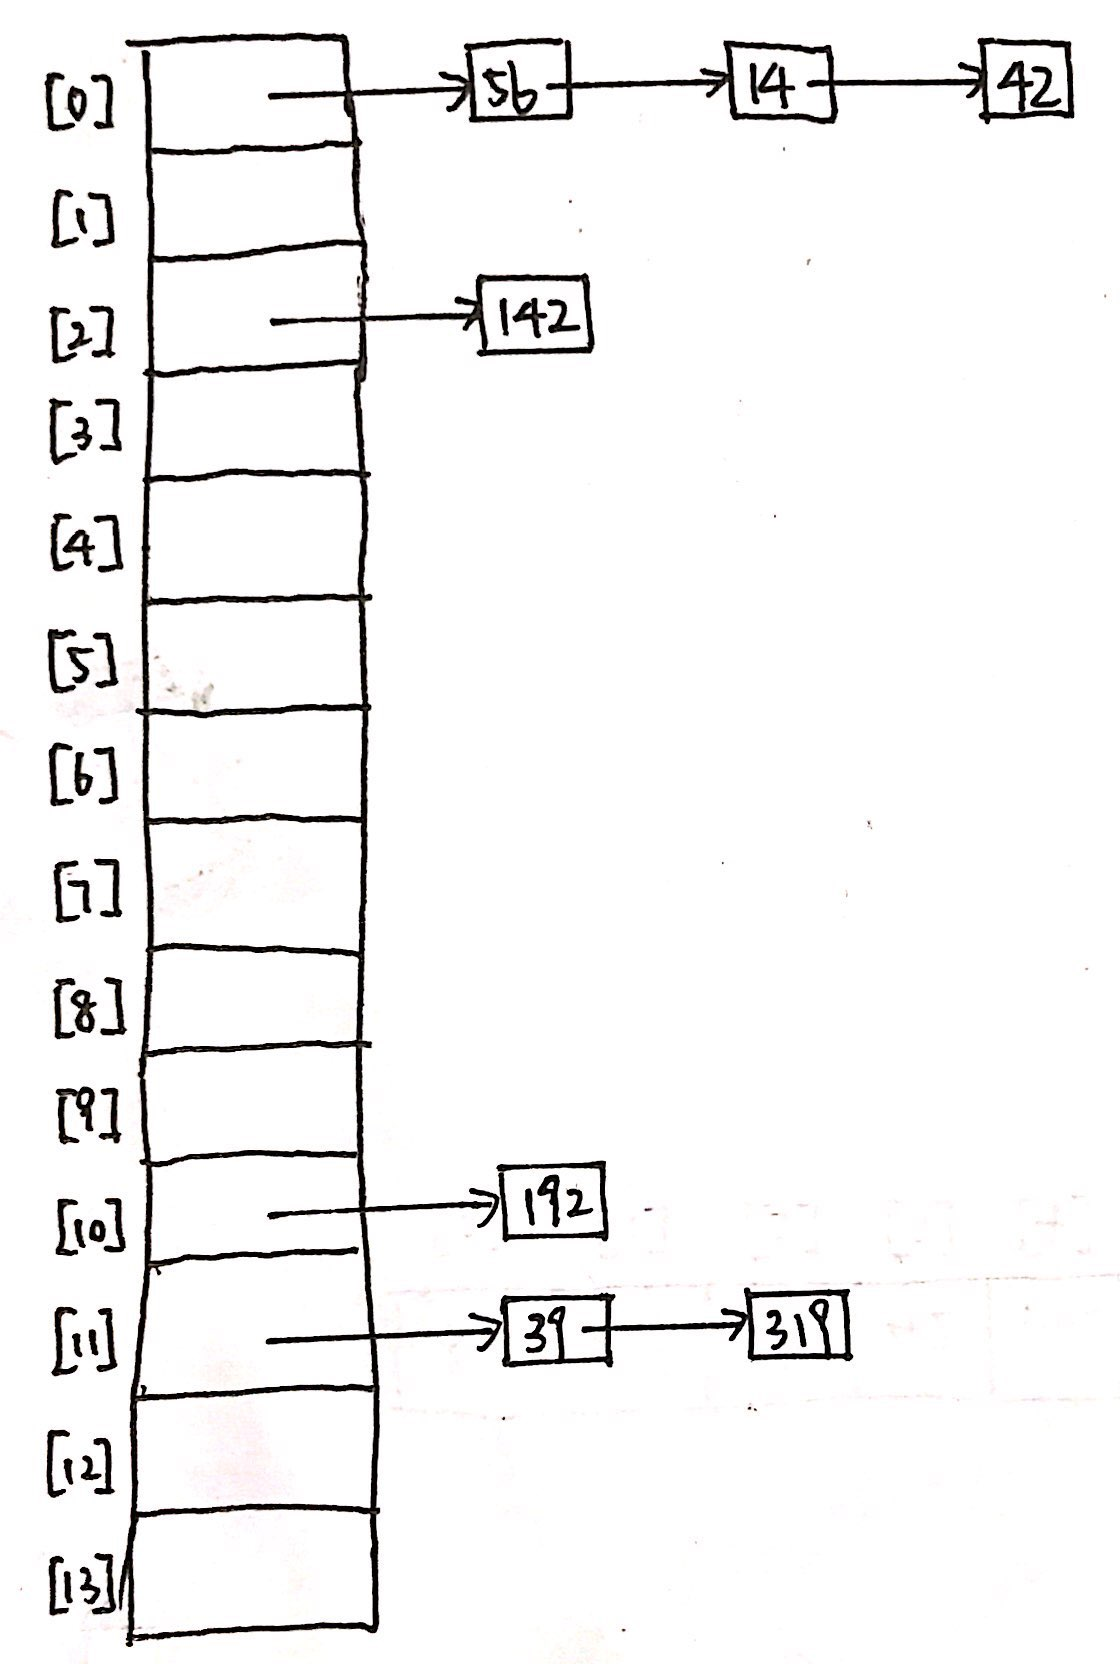
\includegraphics[scale=0.1]{f5.jpg}
	\item Hash table using linear probing.\\
	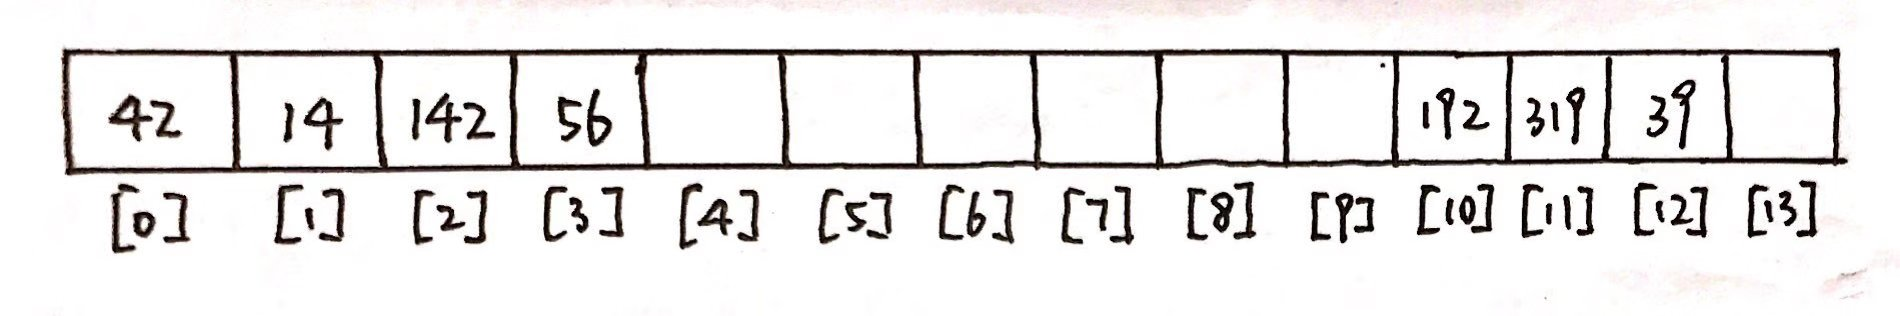
\includegraphics[scale=0.11]{f6.jpg}
	\item Hash table using quadratic probing.\\
	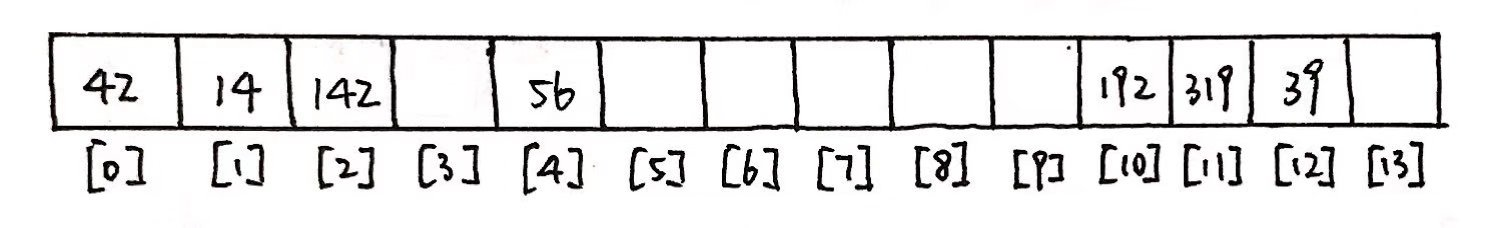
\includegraphics[scale=0.13]{f7.jpg}
	\item Hash table using double hashing, with the second hash function as $h_2 (x) = (x+4)\%7$.\\
	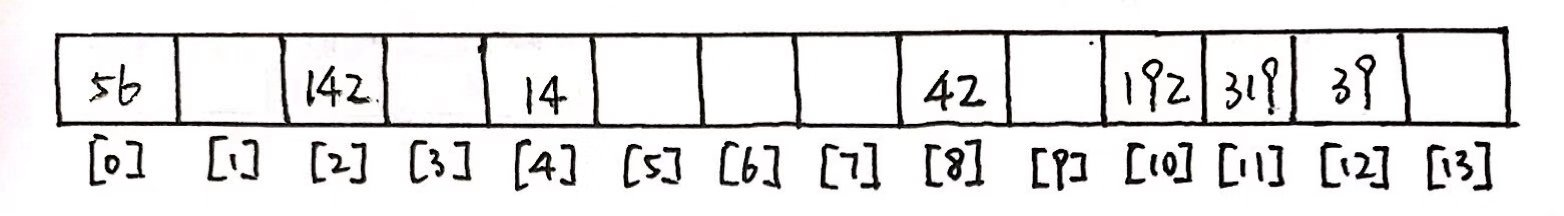
\includegraphics[scale=0.13]{f8.jpg}
	
	\end{enumerate}

\item  Suppose we want to design a hash table containing at most 900 elements using
linear probing. We require that an unsuccessful search needs no more than 8.5 compares
and a successful search needs no more than 3 compares on average. Please determine
a proper hash table size.
\begin{solution}
$$U(L)=\dfrac{1}{2}\left[1+\left(\dfrac{1}{1-L}\right)^2\right]\leq8.5\ \Rightarrow\ L\leq\dfrac{3}{4}$$
$$S(L)=\dfrac{1}{2}\left[1+\dfrac{1}{1-L}\right]\leq3\ \Rightarrow\ L\leq\dfrac{4}{5}$$
$$\therefore L\leq\dfrac{3}{4}$$
$$L=\dfrac{\lvert s\rvert}{n}\leq\dfrac{3}{4}\ \Rightarrow\ n\geq\dfrac{4}{3}\cdot900=1200$$
$$\because\text{We want to pick n as a prime number, }\therefore n=1201$$
\end{solution}

\item Implement queues with two stacks. We know that stacks are first in last out (FILO) and queues are first in first out (FIFO). We can implement queues with two stacks. The method is as follows:
	\begin{itemize}
		\item{For \textbf{enqueue} operation,} push the element into stack $S_1$.
		\item{For \textbf{dequeue} operation,} there are two cases:
		\begin{itemize}
			\item \textbf{$S_2 = \emptyset$,} pop all elements in $S_1$, push these elements into $S_2$, pop $S_2$
			\item \textbf{$S_2 \neq \emptyset$,} pop $S_2$
		\end{itemize}
%$$
%\left\{  
%             \begin{aligned}        
%             &pop all elements in S_1, push these elements in S_2, pop S_2, & S_2 = \emptyset  \\  
%            &pop S_2, &    S_2 \neq \emptyset
%             \end{aligned}  
%\right.  
%$$ 
	\end{itemize}
	Using amortized analysis to calculate the complexity of \textbf{enqueue} and \textbf{dequeue} step.
\begin{solution}
\noindent
\par
Suppose popping an element, pushing an element and checking whether the stack is empty or not each has the complexity of $O(1)$.
\par
Then, total cost of enqueueing $n$ elements is $n\cdot O(1)=O(n)$. Average cost to enqueue an element is $O(1)$.
\par
Suppose the initial state of the two stacks is $S1$ having $n$ elements and $S2$ having no elements inside. Total cost of dequeueing the first $n$ elements is calculated as $n\cdot O(1)+2n\cdot O(1)+n\cdot O(1)=4n\cdot O(1)$, $n\cdot O(1)$ for checking whether $S2$ is empty or not $n$ times, $2n\cdot O(1)$ for popping the $n$ elements out of $S1$ and pushing them into $S2$, $n\cdot O(1)$ for popping them out of $S2$ finally. For the $n+1$-th item, the state of $S1$ and $S2$ return to initial state. Therefore, total cost for dequeueing $n$ items is $4n\cdot O(1)=4O(n)=O(n)$. Average cost to dequeue an element is $O(1)$.
\end{solution}


\end{enumerate}

%========================================================================
\end{document}
